\subsection{Nascent Human and Bovine IFIT Localisation During RSV Infection} \label{subsec:Nascent Human and Bovine IFIT Localisation During RSV Infection}
\subsubsection{Phenotypic Diversity of Nascent IFIT1 Interaction with RSV Inclusion Bodies}
Initial experiment suggested hIFIT1 colocalises with the hRSV IBs in A549 cell line, however assessing all 281 observation we can see that hIFIT1 displays a range of phenotypic divesity with regards to interaction with these structures. As can be seen in Figure \ref{fig:Phenotypic Diversity of hIFIT1 Interactions with hRSV Inclusion Bodies in A549 Cell Line}, panel (a), 30\% of interactions result in either full or partial exclusion from the structure or an even diffusion through the IB and the surroinding cytosol. Next most common phenotype is a inclusion inside the IB structure, occuring in circa 18\% of observation. Following phenotypes, orrucing in the same frequency of 9\%, are a phenotype of colocalisation with the edge of the inclusion body joined with exclusion from the area of the IB; and a edge exclusion phenotype, where IFIT1 was present equaly between the IB and the surrounding cytoplasm with the exeption of of the IB boundry, where its signal is decreased. Representative images of the phenotypes mentioed above can be seen in Figure \ref{fig:Representative Images of Phenotypic Diversity of hIFIT1 Interactions with hRSV Inclusion Bodies in A549 Cell Line}. We have also observed IFIT1 to dysplay edge exclusion with obvoius spots within the IB structure (Edge exclusion + IBAG) and also a colocalisation with phenotype but neither had a sufficiently high frequency of occurance where we can be certain that these are indeed relevant during infection and not just imaging artefacts. In Figure \ref{fig:Phenotypic Diversity of hIFIT1 Interactions with hRSV Inclusion Bodies in A549 Cell Line} panel (b), we can observe the measured areas of the IBs associated with phenotypes which had the frequency of accurance higher than 5\%. We can see that the two most common pheotypes, exclusion and diffusion, had median IB area sizes of 5 and 4.4 \(\mu \mbox{m}^2\), values either identical or very similar to the aggregated median IB area of all the observations in A549 cell line. Both phenotypes also encompass a range of IB sizes, from sub 1 \(\mu \mbox{m}^2\) until supra 20 \(\mu \mbox{m}^2\) IB areas. On the other hand, the other phenotyes observed are more prevalent in larger inclusion bodies. In more detail, inclusion phenotype was more prevalent in supra 3 \(\mu \mbox{m}^2\) inclusion bodies, with the median size of 8; colocalisation accompanied by exclusion phenotype median IB size was 12 \(\mu \mbox{m}^2\), although some IBs with sizes between 0.8 to 5 \(\mu \mbox{m}^2\) showed this phenotype as well; and the edge exlusion phenotype was in IBs with median size of 7 \(\mu \mbox{m}^2\), although these IB were clustered in two clusters with median values of approximately 5 and 10 \(\mu \mbox{m}^2\) respectively. Our data indicates that while in majrity of cases IFIT1 is either excluded or diffused throught the IB structures, regardless ofn the IB size and thus maturity, we can see a potential interaction with more mature IBs of sizes above 5 \(\mu \mbox{m}^2\), which in the literature, coinsides to the IB sizes which have IBAGs present (\cite{Rincheval2017FunctionalVirus}). 

\begin{figure}
    \begin{subfigure}{0.495\textwidth}
        \caption{}
        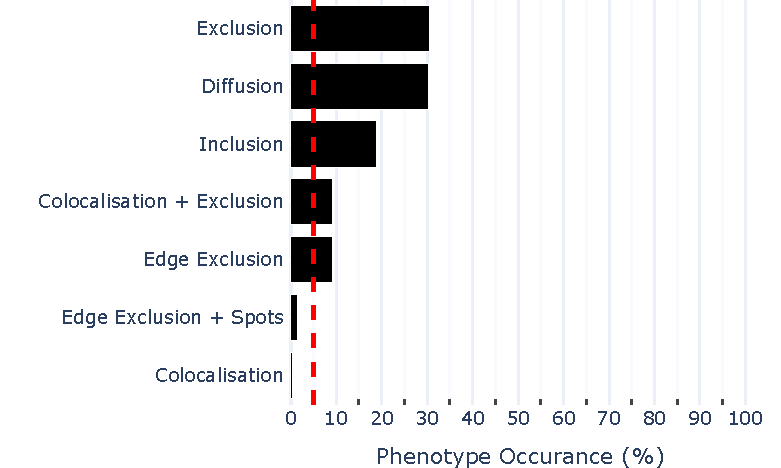
\includegraphics[width=1\linewidth]{08. Chapter 3/Figs/02. Infection/01. IFIT1/01. bar_i1_a549.pdf} 
    \end{subfigure}
    \begin{subfigure}{0.495\textwidth}
        \caption{}
        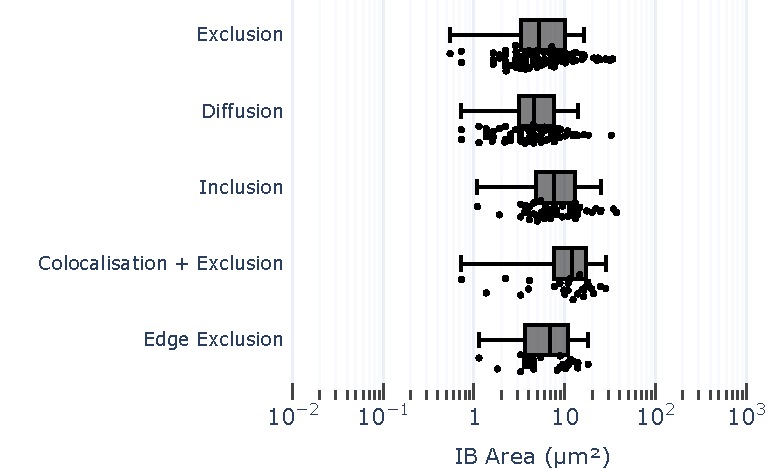
\includegraphics[width=1\linewidth]{08. Chapter 3/Figs/02. Infection/01. IFIT1/02. box_i1_a549.pdf}
    \end{subfigure}
    \caption[Phenotypic Diversity of hIFIT1 Interactions with hRSV Inclusion Bodies in A549 Cell Line.]{\textbf{Phenotypic Diversity of hIFIT1 Interactions with hRSV Inclusion Bodies in A549 Cell Line.} A549 cells were infected with human RSV at MOI 1 and fixed 24 HPI. Cells were double-labeled with with anti-RSV N and anti-IFIT1 antibodies and imaged on confocal microscope. Panel (a) shows percentual proportions of observed phenotypes between hRSV inclusion bodies and hIFIT1 (281 observations), with the red dotted line denoting the 5\% threshold, marking phenotypes considered relevant above this limit. Panel (b) shows the IB area in \(\mu \mbox{m}^2\) per observed relevant phenotype.}
    \label{fig:Phenotypic Diversity of hIFIT1 Interactions with hRSV Inclusion Bodies in A549 Cell Line}
\end{figure}

\begin{figure}
    \centering
    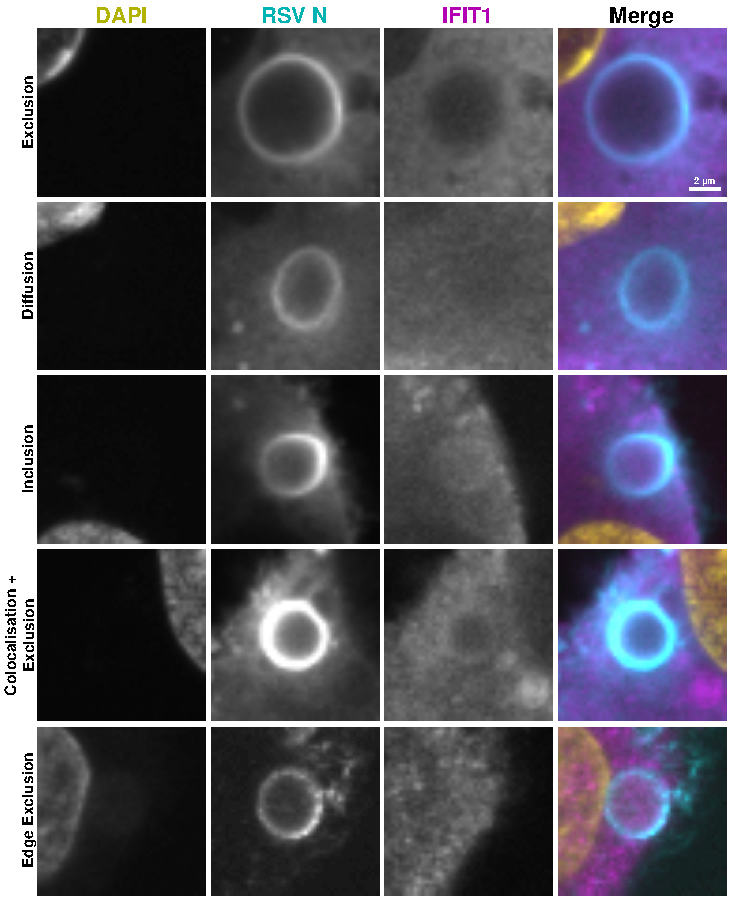
\includegraphics[width=1\linewidth]{08. Chapter 3/Figs/02. Infection/01. IFIT1/03. a549 i1.pdf}
    \caption[Representative Images of Phenotypic Diversity of hIFIT1 Interactions with hRSV Inclusion Bodies in A549 Cell Line.]{\textbf{Representative Images of Phenotypic Diversity of hIFIT1 Interactions with hRSV Inclusion Bodies in A549 Cell Line.} A549 cells were infected with hRSV at MOI 1 and fixed at 24 HPI. Cellular nuclei were stained with DAPI (yellow), and cells were double-labeled with anti-RSV N (cyan) and anti-IFIT1 (magenta) antibodies. This figure showcases representative examples of relevant phenotypes in the interaction between hIFIT1 and hRSV inclusion bodies. These phenotypes are presented in descending order based on their percentage proportions. The scale bar indicates 2 \(\mu \mbox{m}\).}
    \label{fig:Representative Images of Phenotypic Diversity of hIFIT1 Interactions with hRSV Inclusion Bodies in A549 Cell Line}
\end{figure}

We set to validate the previous data in the BEAS2B cell line. Figure \ref{fig:Phenotypic Diversity of hIFIT1 Interactions with hRSV Inclusion Bodies in BEAS2B Cell Line} shows the observed IFIT1/IB interaction phenotypes, their occurance (panel a) and the underlying IB sizes (panel b), while Figure \ref{fig:Representative Images of Phenotypic Diversity of hIFIT1 Interactions with hRSV Inclusion Bodies in BEAS2B Cell Line} shows the respresentative images of phenotypes with the occurance of above 5\%. The majority of observations showed IFIT1 to be either partially or fully excluded from the hRSV inclusion bodies (circa 85\% of observations), while 8\% of phenotypes were diffusion and 4\% displayed colocalisation cojoined with exclusion. The size range of IB from which IFIT1 was exclude mimic the aggregate distribution of all IBs detected within BEAS2B cells, having the equal median size value of 3 \(\mu \mbox{m}^2\) and spread from sub 1 \(\mu \mbox{m}^2\) IBs to supra 10 \(\mu \mbox{m}^2\) ones. The second most common phenotype and the only other that surpassed 5\% of total accurance was diffusion phenitipe, which was observed only in smaller IBs, with the median size of 0.5 \(\mu \mbox{m}^2\).

\begin{figure}
    \begin{subfigure}{0.495\textwidth}
        \caption{}
        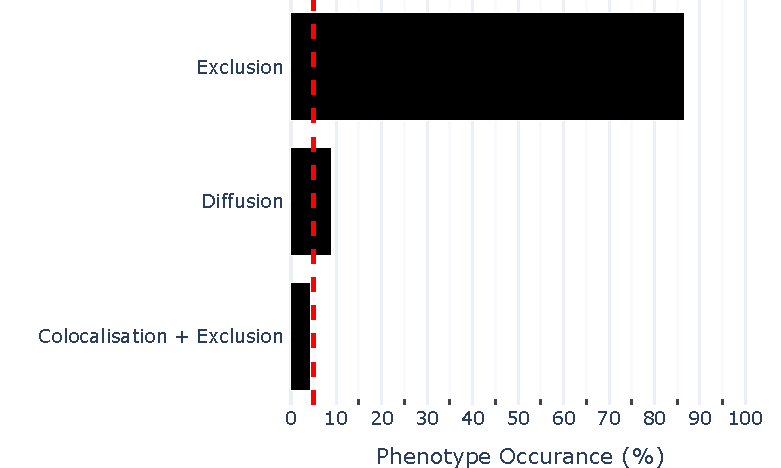
\includegraphics[width=1\linewidth]{08. Chapter 3/Figs/02. Infection/01. IFIT1/04. bar_i1_beas2b.pdf} 
    \end{subfigure}
    \begin{subfigure}{0.495\textwidth}
        \caption{}
        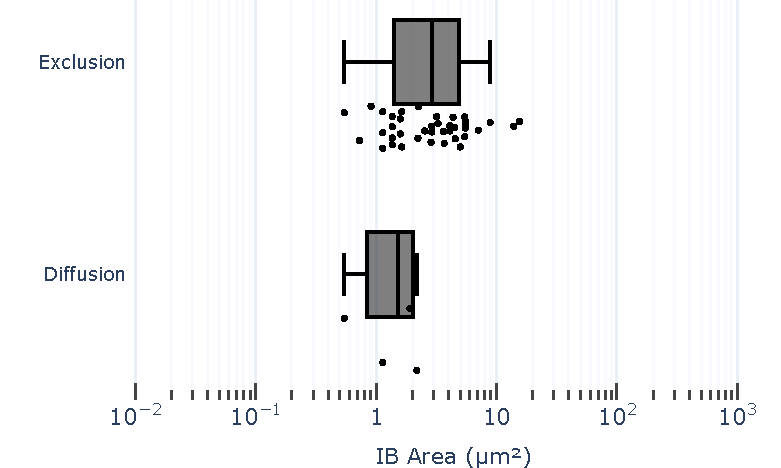
\includegraphics[width=1\linewidth]{08. Chapter 3/Figs/02. Infection/01. IFIT1/05. box_i1_beas2b.pdf}
    \end{subfigure}
    \caption[Phenotypic Diversity of hIFIT1 Interactions with hRSV Inclusion Bodies in BEAS2B Cell Line.]{\textbf{Phenotypic Diversity of hIFIT1 Interactions with hRSV Inclusion Bodies in BEAS2B Cell Line.} BEAS2B cells were infected with human RSV at MOI 1 and fixed 24 HPI. Cells were double-labeled with with anti-RSV N and anti-IFIT1 antibodies and imaged on confocal microscope. Panel (a) shows percentual proportions of observed phenotypes between hRSV inclusion bodies and hIFIT1 (281 observations), with the red dotted line denoting the 5\% threshold, marking phenotypes considered relevant above this limit. Panel (b) shows the IB area in \(\mu \mbox{m}^2\) per observed relevant phenotype.}
    \label{fig:Phenotypic Diversity of hIFIT1 Interactions with hRSV Inclusion Bodies in BEAS2B Cell Line}
\end{figure}

\begin{figure}
    \centering
    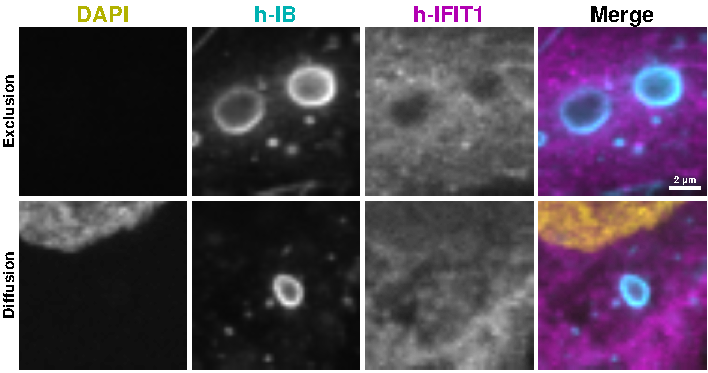
\includegraphics[width=1\linewidth]{08. Chapter 3/Figs/02. Infection/01. IFIT1/06. beas2b i1.pdf}
    \caption[Representative Images of Phenotypic Diversity of hIFIT1 Interactions with hRSV Inclusion Bodies in BEAS2B Cell Line.]{\textbf{Representative Images of Phenotypic Diversity of hIFIT1 Interactions with hRSV Inclusion Bodies in BEAS2B Cell Line.} BEAS2B cells were infected with hRSV at MOI 1 and fixed at 24 HPI. Cellular nuclei were stained with DAPI (yellow), and cells were double-labeled with anti-RSV N (cyan) and anti-IFIT1 (magenta) antibodies. This figure showcases representative examples of relevant phenotypes in the interaction between hIFIT1 and hRSV inclusion bodies. These phenotypes are presented in descending order based on their percentage proportions. The scale bar indicates 2 \(\mu \mbox{m}\).}
    \label{fig:Representative Images of Phenotypic Diversity of hIFIT1 Interactions with hRSV Inclusion Bodies in BEAS2B Cell Line}
\end{figure}

Lastly we investigated the behaviour of bovine IFIT1 during bRSV infection. Figure \ref{fig:Phenotypic Diversity of bIFIT1 Interactions with bRSV Inclusion Bodies in MDBK Cell Line} higlights the phynotipic diversity in detail. Similar to what was observed in A549 and BEAS2B cell line, the most common phenotype with around 65\% frequency is exclusion, however, the second most common one is intra IB inclusion (around 23\%). This is followed by diffusion phenotype, and edge exclusion without or with the presence of possible IBAGs. Out of these, only diffusion was observed with at least 5\% frequency. The representative images of phenotypes with frequency of occurance above 5\% are presented in Figure \ref{fig:Representative Images of Phenotypic Diversity of bIFIT1 Interactions with bRSV Inclusion Bodies in MDBK Cell Line}. In terms of the IB size profile during each observed phenotype, the exclusion-associated IBs had the mean size of 2 \(\mu \mbox{m}\), with the sizes ranging from sub 0.5 \(\mu \mbox{m}\) to supra 30 \(\mu \mbox{m}\), comparable with the median values on overal distribution of the aggregate IB size values detected in MDBK cell line. The inclusion clustered in two size ranges, predominantly to IBs with the size of around 0.9 \(\mu \mbox{m}\), and to IBs with the sizes above 10 \(\mu \mbox{m}\). Lastly, we observed the diffusion phenotype to occur in IBs from 0.2 \(\mu \mbox{m}\) to around 7 \(\mu \mbox{m}\), with the median value of 1.3 \(\mu \mbox{m}\).

COMPARE AND CONTRAST ALL IFIT1 IN ALL 3 CELL LINES

\begin{figure}
    \begin{subfigure}{0.495\textwidth}
        \caption{}
        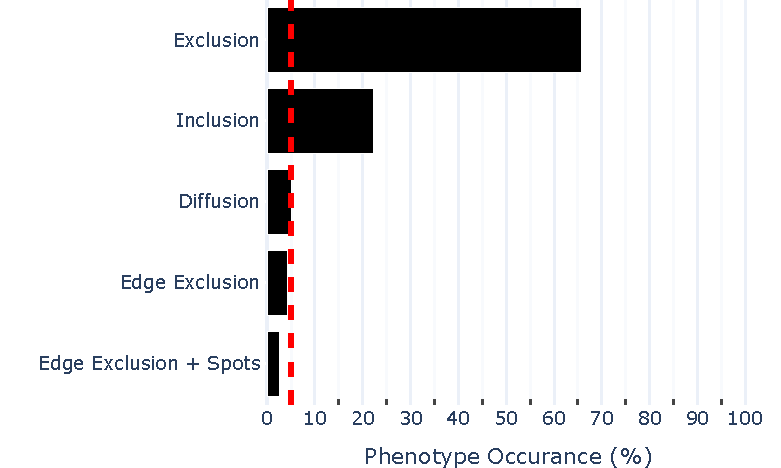
\includegraphics[width=1\linewidth]{08. Chapter 3/Figs/02. Infection/01. IFIT1/07. bar_i1_mdbk.pdf} 
    \end{subfigure}
    \begin{subfigure}{0.495\textwidth}
        \caption{}
        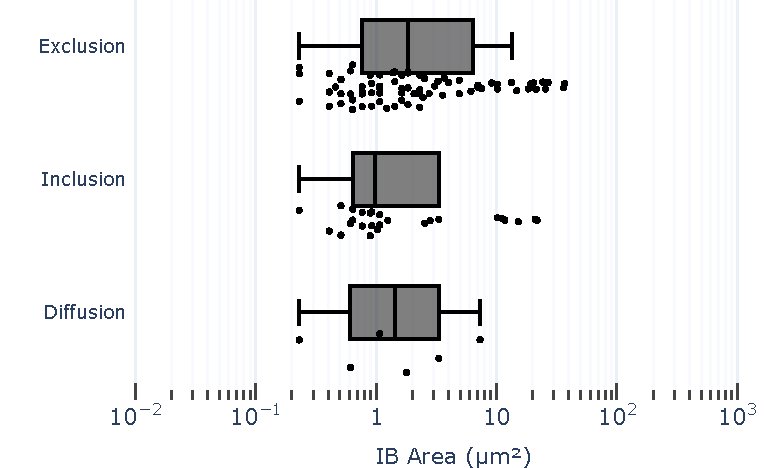
\includegraphics[width=1\linewidth]{08. Chapter 3/Figs/02. Infection/01. IFIT1/08. box_i1_mdbk.pdf}
    \end{subfigure}
    \caption[Phenotypic Diversity of bIFIT1 Interactions with bRSV Inclusion Bodies in MDBK Cell Line.]{\textbf{Phenotypic Diversity of bIFIT1 Interactions with bRSV Inclusion Bodies in MDBK Cell Line.} MDBK cells were infected with bovine RSV at MOI 1 and fixed 24 HPI. Cells were double-labeled with with anti-RSV N and anti-IFIT1 antibodies and imaged on confocal microscope. Panel (a) shows percentual proportions of observed phenotypes between bRSV inclusion bodies and bIFIT1 (117 observations), with the red dotted line denoting the 5\% threshold, marking phenotypes considered relevant above this limit. Panel (b) shows the IB area in \(\mu \mbox{m}^2\) per observed relevant phenotype.}
    \label{fig:Phenotypic Diversity of bIFIT1 Interactions with bRSV Inclusion Bodies in MDBK Cell Line}
\end{figure}

\begin{figure}
    \centering
    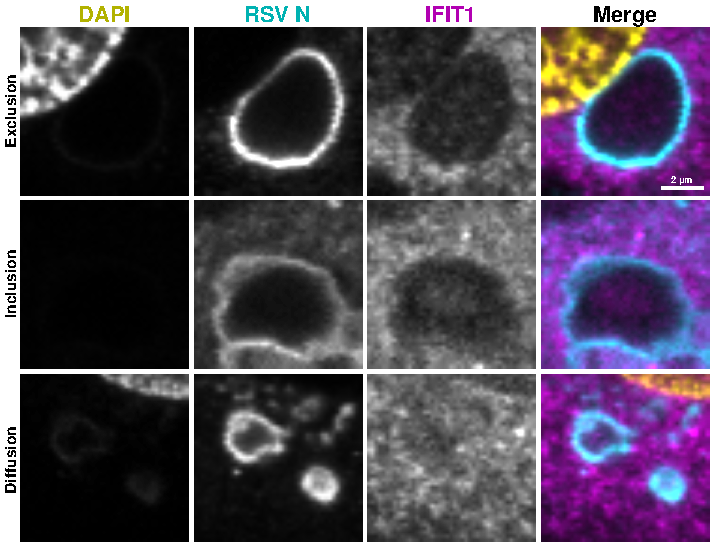
\includegraphics[width=1\linewidth]{08. Chapter 3/Figs/02. Infection/01. IFIT1/09. mdbk i1.pdf}
    \caption[Representative Images of Phenotypic Diversity of bIFIT1 Interactions with bRSV Inclusion Bodies in MDBK Cell Line.]{\textbf{Representative Images of Phenotypic Diversity of bIFIT1 Interactions with bRSV Inclusion Bodies in MDBK Cell Line.} MDBK cells were infected with bRSV at MOI 1 and fixed at 24 HPI. Cellular nuclei were stained with DAPI (yellow), and cells were double-labeled with anti-RSV N (cyan) and anti-IFIT1 (magenta) antibodies. This figure showcases representative examples of relevant phenotypes in the interaction between bIFIT1 and bRSV inclusion bodies. These phenotypes are presented in descending order based on their percentage proportions. The scale bar indicates 2 \(\mu \mbox{m}\).}
    \label{fig:Representative Images of Phenotypic Diversity of bIFIT1 Interactions with bRSV Inclusion Bodies in MDBK Cell Line}
\end{figure}

\subsubsection{Phenotypic Diversity of Nascent IFIT2 Interaction with RSV Inclusion Bodies}
As described in Section \ref{subsec:IFIT Subcellular Localisation During Interferon Induction and RSV Infection}, we utilised two antibodies against IFIT2 protein, which yielded differential results with regards to both subcellular localisation and the interaction phenotype with the RSV IBs. With the latter IFIT2A antibody showed IFIT2 to form intra IB inclusions in A549 cell line, while it show IFIT2 to colocalise with the bRSV IB boundry, while being excluded from this structure. On the other hand, IFIT2B antibody showed exclusion of both human and bovine IFIT2 from the IB structures. We examined these interactions in more detail bellow.

The results of the phenotypic diversity of the interactions of IFIT2 proteins in A549 cell line with hRSV IBs, as detected by the IFIT2A antibody, can be seen in the Figure \ref{fig:Phenotypic Diversity of hIFIT2 Interactions with hRSV Inclusion Bodies, Detected by IFIT2A Antibody in A549 Cell Line}. The examples of the phenotypic interactions are shown in Figure \ref{fig:Representative Images of Phenotypic Diversity of hIFIT2 Interactions with hRSV Inclusion Bodies, Detected by IFIT2A Antibody in A549 Cell Line}. We can see that the most common phenotype, occuring with frequency of around 70\%, is intra IB inclusion. This aligns with our observations from Section \ref{subsec:IFIT Subcellular Localisation During Interferon Induction and RSV Infection} (Figure \ref{fig:The Changes in Subcellular Localisation of Human IFITs in A549 Cells Subjected to hIFNa or hRSV}), however we see additional interactions to occur as well. Colocalisation accompanied by exclusion occurs in 30\% of observations, while an exclusion phenotype occured in 1\% of observations. In terms of the measured areas of the IBs in which the differential interaction phenotypes occure with at least 5\% frequency, we can see that the inclusion and colocalisation accompanied by IB exclusion phenotypes clustered into two almost exclusive groups. The former had the median area of 2.1 \(\mu \mbox{m}\), which was lower than the median area of all A549 IB observations (which had median value of 5 \(\mu \mbox{m}\)), while the latter occured in larger Ibs, with the median size of 9 \(\mu \mbox{m}\). It should be noted that there is a ovelap in terms of the sizes of IBs with either phenotype, however, this data sugegst IFIT2 forming predominantly inclusions in imature IBs with its interaction shifting to IB boundry colocalisation with accompanied IB exclusion in the more mature IBs.

\begin{figure}
    \begin{subfigure}{0.495\textwidth}
        \caption{}
        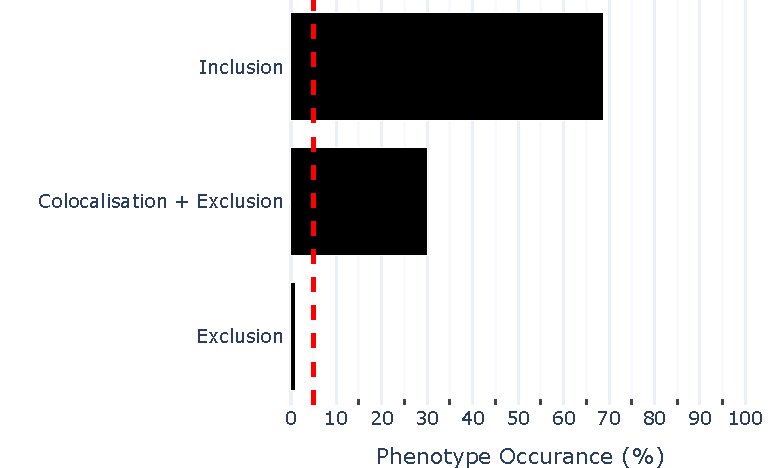
\includegraphics[width=1\linewidth]{08. Chapter 3/Figs/02. Infection/02. IFIT2/01. IFIT2A/01. bar_i2a_a549.pdf}
    \end{subfigure}
    \begin{subfigure}{0.495\textwidth}
        \caption{}
        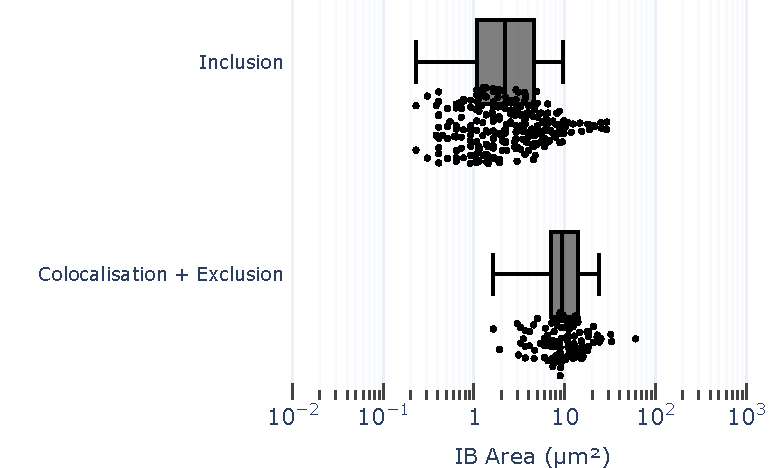
\includegraphics[width=1\linewidth]{08. Chapter 3/Figs/02. Infection/02. IFIT2/01. IFIT2A/02. box_i2a_a549.pdf}
    \end{subfigure}
    \caption[Phenotypic Diversity of hIFIT2 Interactions with hRSV Inclusion Bodies, Detected by IFIT2A Antibody in A549 Cell Line.]{\textbf{Phenotypic Diversity of hIFIT2 Interactions with hRSV Inclusion Bodies, Detected by IFIT2A Antibody in A549 Cell Line.} A549 cells were infected with human RSV at MOI 1 and fixed 24 HPI. Cells were labeled with anti-RSV N and anti-IFIT2A antibodies and imaged on confocal microscope. Panel (a) shows percentual proportions of observed phenotypes between hRSV inclusion bodies and hIFIT2, detected by IFIT2A antibody (340 observations), with the red dotted line denoting the 5\% threshold, marking phenotypes considered relevant above this limit. Panel (b) shows the IB area in \(\mu \mbox{m}^2\) per observed relevant phenotype.}
    \label{fig:Phenotypic Diversity of hIFIT2 Interactions with hRSV Inclusion Bodies, Detected by IFIT2A Antibody in A549 Cell Line}
\end{figure}

\begin{figure}
    \centering
    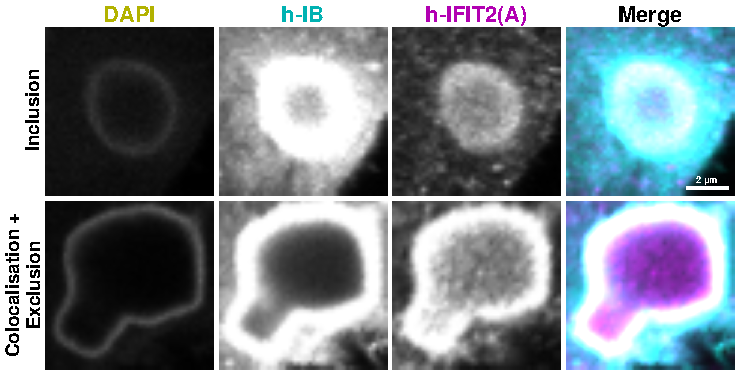
\includegraphics[width=1\linewidth]{08. Chapter 3/Figs/02. Infection/02. IFIT2/01. IFIT2A/03. i2a-a549.pdf}
    \caption[Representative Images of Phenotypic Diversity of hIFIT2 Interactions with hRSV Inclusion Bodies, Detected by IFIT2A Antibody in A549 Cell Line.]{\textbf{Representative Images of Phenotypic Diversity of hIFIT2 Interactions with hRSV Inclusion Bodies, Detected by IFIT2A Antibody in A549 Cell Line.} A549 cells were infected with hRSV at MOI 1 and fixed at 24 HPI. Cellular nuclei were stained with DAPI (yellow), and cells were double-labeled with anti-RSV N (cyan) and anti-IFIT2A (magenta) antibodies. This figure showcases representative examples of relevant phenotypes in the interaction between hIFIT2, detected by IFIT2A antibody, and hRSV inclusion bodies. These phenotypes are presented in descending order based on their percentage proportions. The scale bar indicates 2 \(\mu \mbox{m}\).}
    \label{fig:Representative Images of Phenotypic Diversity of hIFIT2 Interactions with hRSV Inclusion Bodies, Detected by IFIT2A Antibody in A549 Cell Line}
\end{figure}

For IFIT2 interaction phenotypes with hRSV IBs, as detected by the IFIT2B antibody, we observe it to conform to our previous observations from Section \ref{subsec:IFIT Subcellular Localisation During Interferon Induction and RSV Infection} (Figure \ref{fig:The Changes in Subcellular Localisation of Human IFITs in A549 Cells Subjected to hIFNa or hRSV} and Figure \ref{fig:The Changes in Subcellular Localisation of Bovine IFITs in MDBK Cells Subjected to bIFNa or bRSV}). The underlyig phenotype frequence data, along with the measired IB sizes can be seen in Figure \ref{fig:Phenotypic Diversity of hIFIT2 Interactions with hRSV Inclusion Bodies, Detected by IFIT2B Antibody in A549 Cell Line}, while the representative images of the major occuring phenotype can be seen in Figure \ref{fig:Representative Images of Phenotypic Diversity of hIFIT2 Interactions with hRSV Inclusion Bodies, Detected by IFIT2B Antibody in A549 Cell Line}. We can see that in 97\% of IB occurances, IFIT2 was found to be excluded from the structure. 3\% of the observations showed IFIT2 to be excluded through both cytoplasm and the IB structure. In terms of the size profile of the exclusion-associated IBs, they have a minimal size of 4 \(\mu \mbox{m}^2\), median size of 5 \(\mu \mbox{m}^2\), and maximal observed size of supra 30 \(\mu \mbox{m}^2\). This distribution is neraly identical to the aggregate distribution of all IBs detected in A549 in this study (Section \ref{subsec:IFIT Subcellular Localisation During Interferon Induction and RSV Infection}, Figure \ref{fig:The Distributions of IB Areas Observed Per Cell Line}), which allows us to confirm that IFIT2, as detected by the IFIT2B antibody in A549 cell line, is excluded from these structures regardless of the IB size and thus maturity and these results are not a result of observational bias.

\begin{figure}
    \begin{subfigure}{0.495\textwidth}
        \caption{}
        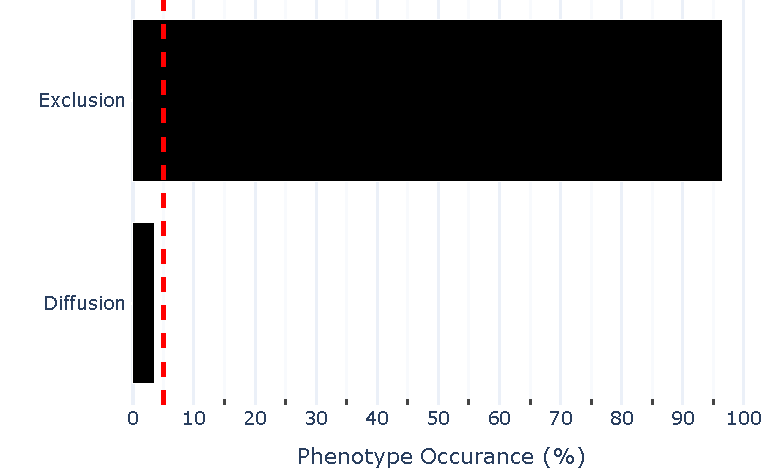
\includegraphics[width=1\linewidth]{08. Chapter 3/Figs/02. Infection/02. IFIT2/02. IFIT2B/01. bar_i2b_a549.pdf}
    \end{subfigure}
    \begin{subfigure}{0.495\textwidth}
        \caption{}
        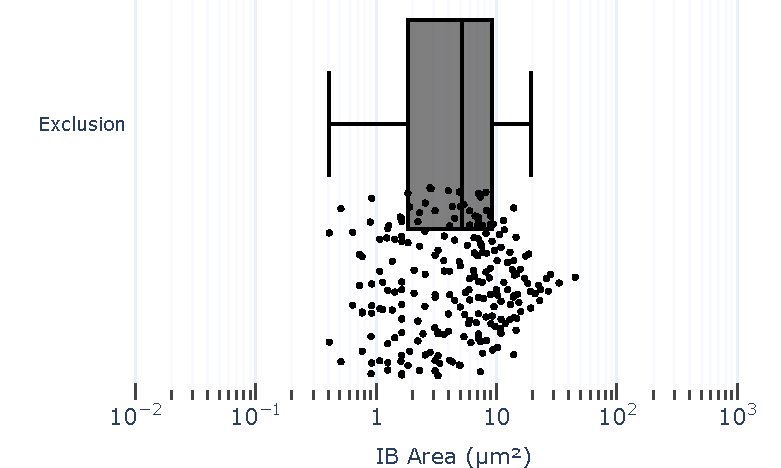
\includegraphics[width=1\linewidth]{08. Chapter 3/Figs/02. Infection/02. IFIT2/02. IFIT2B/02. box_i2b_a549.pdf}
    \end{subfigure}
    \caption[Phenotypic Diversity of hIFIT2 Interactions with hRSV Inclusion Bodies, Detected by IFIT2B Antibody in A549 Cell Line.]{\textbf{Phenotypic Diversity of hIFIT2 Interactions with hRSV Inclusion Bodies, Detected by IFIT2B Antibody in A549 Cell Line.} A549 cells were infected with human RSV at MOI 1 and fixed 24 HPI. Cells were labeled with anti-RSV N and anti-IFIT2B antibodies and imaged on confocal microscope. Panel (a) shows percentual proportions of observed phenotypes between hRSV inclusion bodies and hIFIT2, detected by IFIT2B antibody (230 observations), with the red dotted line denoting the 5\% threshold, marking phenotypes considered relevant above this limit. Panel (b) shows the IB area in \(\mu \mbox{m}^2\) per observed relevant phenotype.}
    \label{fig:Phenotypic Diversity of hIFIT2 Interactions with hRSV Inclusion Bodies, Detected by IFIT2B Antibody in A549 Cell Line}
\end{figure}

\begin{figure}
    \centering
    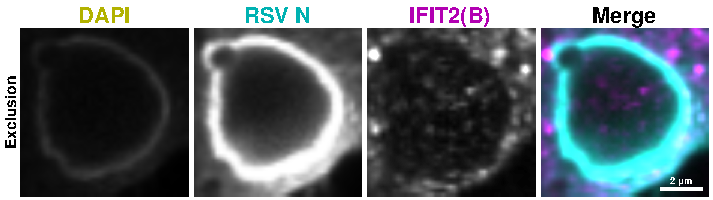
\includegraphics[width=1\linewidth]{08. Chapter 3/Figs/02. Infection/02. IFIT2/02. IFIT2B/03. i2b-a549.pdf} 
    \caption[Representative Images of Phenotypic Diversity of hIFIT2 Interactions with hRSV Inclusion Bodies, Detected by IFIT2B Antibody in A549 Cell Line.]{\textbf{Representative Images of Phenotypic Diversity of hIFIT2 Interactions with hRSV Inclusion Bodies, Detected by IFIT2B Antibody in A549 Cell Line.} A549 cells were infected with hRSV at MOI 1 and fixed at 24 HPI. Cellular nuclei were stained with DAPI (yellow), and cells were double-labeled with anti-RSV N (cyan) and anti-IFIT2B (magenta) antibodies. This figure showcases representative examples of relevant phenotypes in the interaction between hIFIT2, detected by IFIT2B antibody, and hRSV inclusion bodies. These phenotypes are presented in descending order based on their percentage proportions. The scale bar indicates 2 \(\mu \mbox{m}\).}
    \label{fig:Representative Images of Phenotypic Diversity of hIFIT2 Interactions with hRSV Inclusion Bodies, Detected by IFIT2B Antibody in A549 Cell Line}
\end{figure}

Seeing that the IFIT2A antibody showed results of human IFIT2 localisations not observed presiously in our study, while IFIT2B antibody showed results that were consistent with our previous data (both refering to the data from section \ref{subsec:IFIT Subcellular Localisation During Interferon Induction and RSV Infection}, Figure \ref{fig:The Changes in Subcellular Localisation of Human IFITs in A549 Cells Subjected to hIFNa or hRSV}), we decided to validate the IFIT2A results unsing BEA2B cell line infected with hRSV at MOI 1. Smaples were fixed 24 HPI. The phenotipic diversity data can be seen in Figure \ref{fig:Phenotypic Diversity of hIFIT2 Interactions with hRSV Inclusion Bodies, Detected by IFIT2A Antibody in BEAS2B Cell Line}, while the representative images of these phenotypes are shown in Figure \ref{fig:Representative Images of Phenotypic Diversity of hIFIT2 Interactions with hRSV Inclusion Bodies, Detected by IFIT2A Antibody in BEAS2B Cell Line}.

DESCRIBE THE DATA

71 21 6

2.1 8 15

Put all human i2 data togehter

\begin{figure}
    \begin{subfigure}{0.495\textwidth}
        \caption{}
        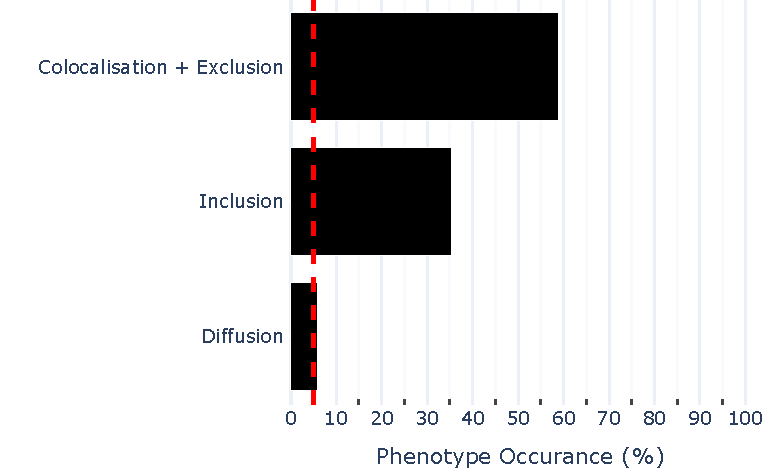
\includegraphics[width=1\linewidth]{08. Chapter 3/Figs/02. Infection/02. IFIT2/01. IFIT2A/10. bar_i2a_beas2b.pdf} 
    \end{subfigure}
    \begin{subfigure}{0.495\textwidth}
        \caption{}
        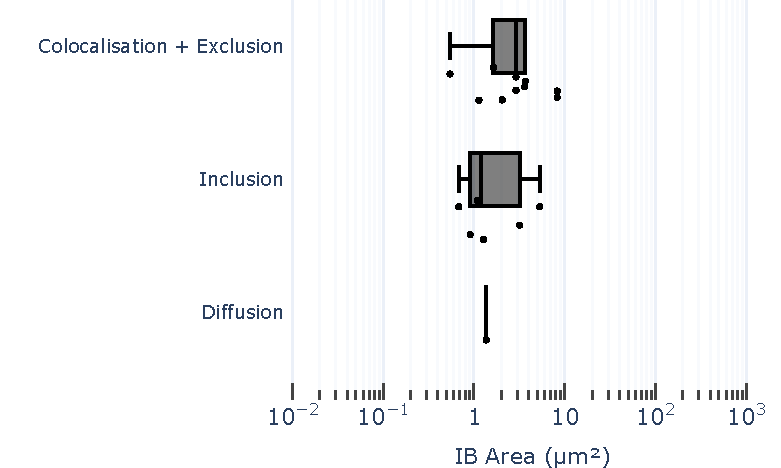
\includegraphics[width=1\linewidth]{08. Chapter 3/Figs/02. Infection/02. IFIT2/01. IFIT2A/11. box_i2a_beas2b.pdf}
    \end{subfigure}
    \caption[Phenotypic Diversity of hIFIT2 Interactions with hRSV Inclusion Bodies, Detected by IFIT2A Antibody in BEAS2B Cell Line.]{\textbf{Phenotypic Diversity of hIFIT2 Interactions with hRSV Inclusion Bodies, Detected by IFIT2A Antibody in BEAS2B Cell Line.} BEAS2B cells were infected with human RSV at MOI 1 and fixed 24 HPI. Cells were labeled with anti-RSV N and anti-IFIT2A antibodies and imaged on confocal microscope. Panel (a) shows percentual proportions of observed phenotypes between hRSV inclusion bodies and hIFIT2, detected by IFIT2A antibody (99 observations), with the red dotted line denoting the 5\% threshold, marking phenotypes considered relevant above this limit. Panel (b) shows the IB area in \(\mu \mbox{m}^2\) per observed relevant phenotype.}
    \label{fig:Phenotypic Diversity of hIFIT2 Interactions with hRSV Inclusion Bodies, Detected by IFIT2A Antibody in BEAS2B Cell Line}
\end{figure}

\begin{figure}
    \centering
    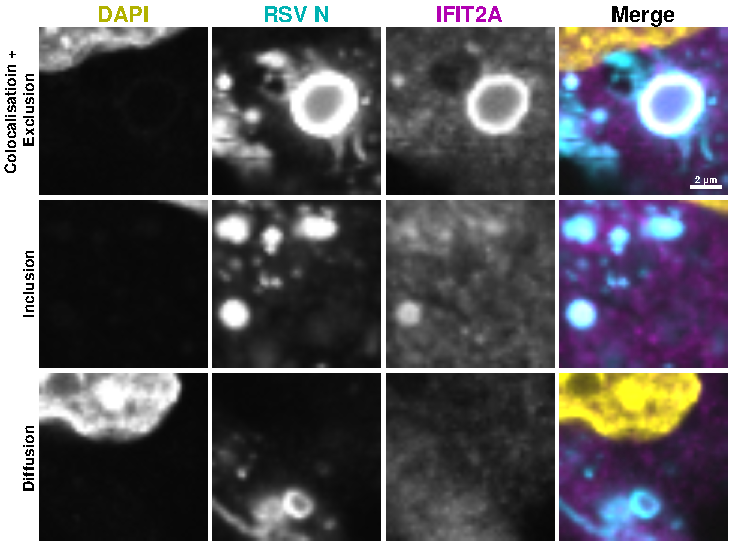
\includegraphics[width=1\linewidth]{08. Chapter 3/Figs/02. Infection/02. IFIT2/01. IFIT2A/12. i2a beas2b.pdf} 
    \caption[Representative Images of Phenotypic Diversity of hIFIT2 Interactions with hRSV Inclusion Bodies, Detected by IFIT2A Antibody in BEAS2B Cell Line.]{\textbf{Representative Images of Phenotypic Diversity of hIFIT2 Interactions with hRSV Inclusion Bodies, Detected by IFIT2A Antibody in BEAS2B Cell Line.} BEAS2B cells were infected with hRSV at MOI 1 and fixed at 24 HPI. Cellular nuclei were stained with DAPI (yellow), and cells were double-labeled with anti-RSV N (cyan) and anti-IFIT2A (magenta) antibodies. This figure showcases representative examples of relevant phenotypes in the interaction between hIFIT2, detected by IFIT2A antibody, and hRSV inclusion bodies. These phenotypes are presented in descending order based on their percentage proportions. The scale bar indicates 2 \(\mu \mbox{m}\).}
    \label{fig:Representative Images of Phenotypic Diversity of hIFIT2 Interactions with hRSV Inclusion Bodies, Detected by IFIT2A Antibody in BEAS2B Cell Line}
\end{figure}

I2A MDBK DATA

58 35 5

3 1.2 1.2


\begin{figure}
    \begin{subfigure}{0.495\textwidth}
        \caption{}
        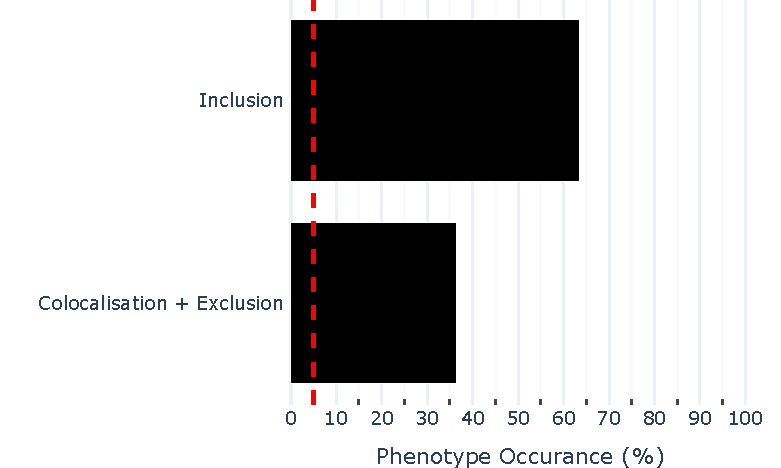
\includegraphics[width=1\linewidth]{08. Chapter 3/Figs/02. Infection/02. IFIT2/01. IFIT2A/13. bar_i2a_mdbk.pdf} 
    \end{subfigure}
    \begin{subfigure}{0.495\textwidth}
        \caption{}
        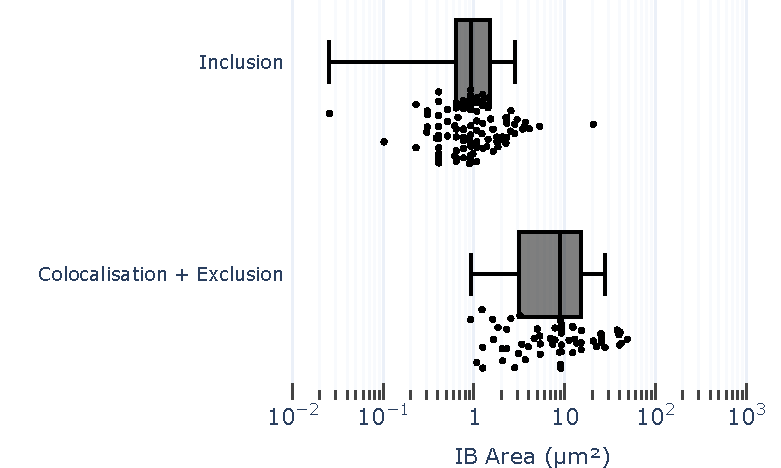
\includegraphics[width=1\linewidth]{08. Chapter 3/Figs/02. Infection/02. IFIT2/01. IFIT2A/14. box_i2a_mdbk.pdf}
    \end{subfigure}
    \caption[Phenotypic Diversity of hIFIT2 Interactions with bRSV Inclusion Bodies, Detected by IFIT2A Antibody in MDBK Cell Line.]{\textbf{Phenotypic Diversity of hIFIT2 Interactions with bRSV Inclusion Bodies, Detected by IFIT2A Antibody in MDBK Cell Line.} MDBK cells were infected with bovine RSV at MOI 1 and fixed 24 HPI. Cells were labeled with anti-RSV N and anti-IFIT2A antibodies and imaged on confocal microscope. Panel (a) shows percentual proportions of observed phenotypes between bRSV inclusion bodies and bIFIT2, detected by IFIT2A antibody (162 observations), with the red dotted line denoting the 5\% threshold, marking phenotypes considered relevant above this limit. Panel (b) shows the IB area in \(\mu \mbox{m}^2\) per observed relevant phenotype.}
    \label{fig:Phenotypic Diversity of hIFIT2 Interactions with bRSV Inclusion Bodies, Detected by IFIT2A Antibody in MDBK Cell Line}
\end{figure}

\begin{figure}
    \centering
    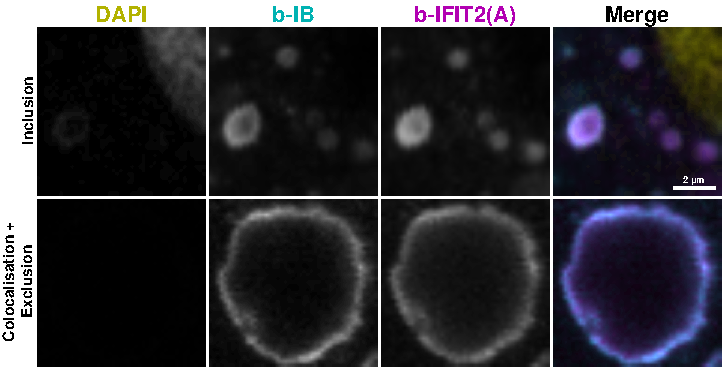
\includegraphics[width=1\linewidth]{08. Chapter 3/Figs/02. Infection/02. IFIT2/01. IFIT2A/15. i2a mdbk brsv.pdf} 
    \caption[Representative Images of Phenotypic Diversity of hIFIT2 Interactions with bRSV Inclusion Bodies, Detected by IFIT2A Antibody in MDBK Cell Line.]{\textbf{Representative Images of Phenotypic Diversity of hIFIT2 Interactions with bRSV Inclusion Bodies, Detected by IFIT2A Antibody in MDBK Cell Line.} MDBK cells were infected with bRSV at MOI 1 and fixed at 24 HPI. Cellular nuclei were stained with DAPI (yellow), and cells were double-labeled with anti-RSV N (cyan) and anti-IFIT2A (magenta) antibodies. This figure showcases representative examples of relevant phenotypes in the interaction between bIFIT2, detected by IFIT2A antibody, and bRSV inclusion bodies. These phenotypes are presented in descending order based on their percentage proportions. The scale bar indicates 2 \(\mu \mbox{m}\).}
    \label{fig:Representative Images of Phenotypic Diversity of hIFIT2 Interactions with bRSV Inclusion Bodies, Detected by IFIT2A Antibody in MDBK Cell Line}
\end{figure}

I2B MDBK DATA

64 36

1 9

PUT ALL IFIT2 MDBK TOGETHER 

PUT ALL IFIT2 DATA TOGETHER FROM ALL 3 CELL LINES

\begin{figure}
    \begin{subfigure}{0.495\textwidth}
        \caption{}
        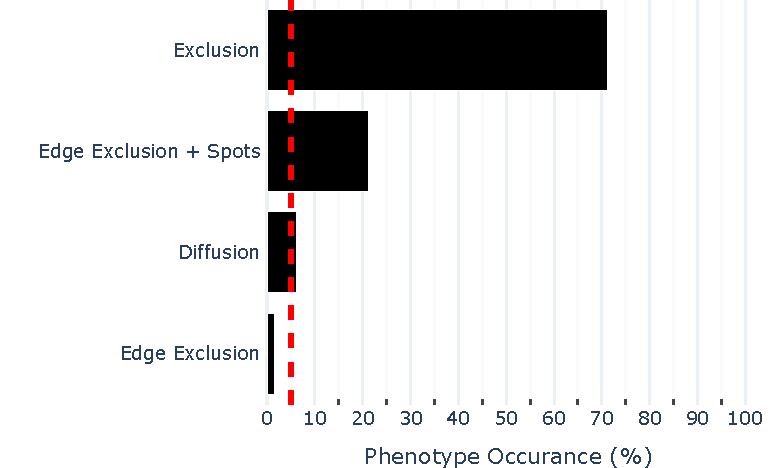
\includegraphics[width=1\linewidth]{08. Chapter 3/Figs/02. Infection/02. IFIT2/02. IFIT2B/10. bar_i2b_mdbk.pdf} 
    \end{subfigure}
    \begin{subfigure}{0.495\textwidth}
        \caption{}
        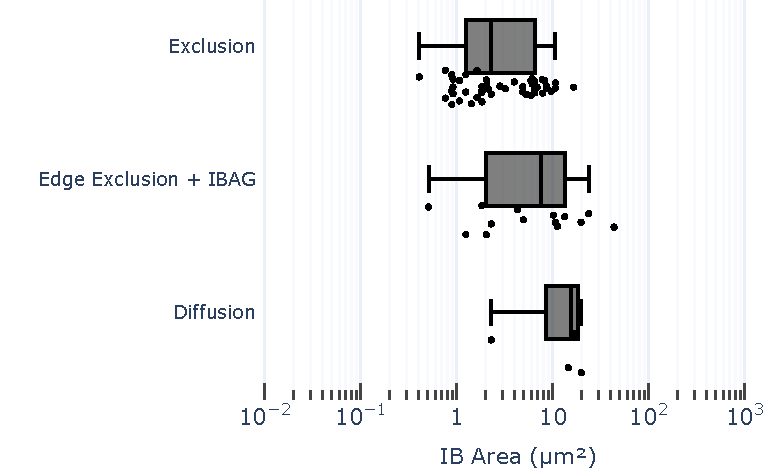
\includegraphics[width=1\linewidth]{08. Chapter 3/Figs/02. Infection/02. IFIT2/02. IFIT2B/11. box_i2b_mdbk.pdf}
    \end{subfigure}
    \caption[Phenotypic Diversity of hIFIT2 Interactions with bRSV Inclusion Bodies, Detected by IFIT2B Antibody in MDBK Cell Line.]{\textbf{Phenotypic Diversity of hIFIT2 Interactions with bRSV Inclusion Bodies, Detected by IFIT2B Antibody in MDBK Cell Line.} MDBK cells were infected with bovine RSV at MOI 1 and fixed 24 HPI. Cells were labeled with anti-RSV N and anti-IFIT2B antibodies and imaged on confocal microscope. Panel (a) shows percentual proportions of observed phenotypes between bRSV inclusion bodies and bIFIT2, detected by IFIT2B antibody (66 observations), with the red dotted line denoting the 5\% threshold, marking phenotypes considered relevant above this limit. Panel (b) shows the IB area in \(\mu \mbox{m}^2\) per observed relevant phenotype.}
    \label{fig:Phenotypic Diversity of hIFIT2 Interactions with bRSV Inclusion Bodies, Detected by IFIT2B Antibody in MDBK Cell Line}
\end{figure}

\begin{figure}
    \centering
    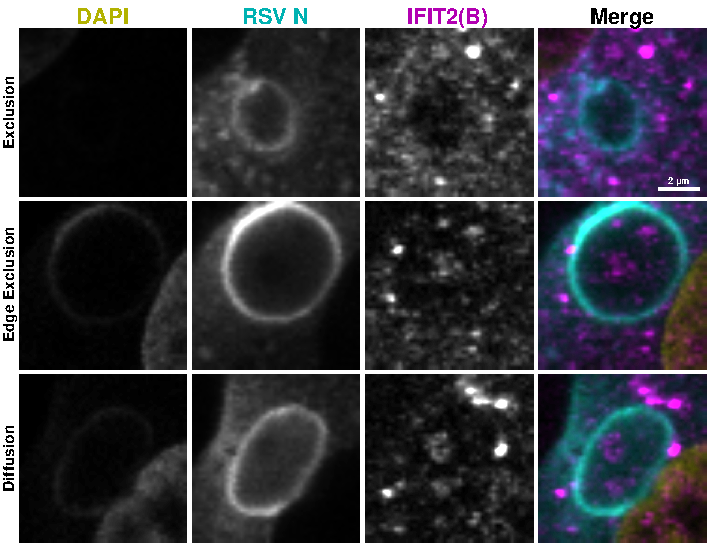
\includegraphics[width=1\linewidth]{08. Chapter 3/Figs/02. Infection/02. IFIT2/02. IFIT2B/12. i2b mdbk brsv.pdf} 
    \caption[Representative Images of Phenotypic Diversity of hIFIT2 Interactions with bRSV Inclusion Bodies, Detected by IFIT2B Antibody in MDBK Cell Line.]{\textbf{Representative Images of Phenotypic Diversity of hIFIT2 Interactions with bRSV Inclusion Bodies, Detected by IFIT2B Antibody in MDBK Cell Line.} MDBK cells were infected with bRSV at MOI 1 and fixed at 24 HPI. Cellular nuclei were stained with DAPI (yellow), and cells were double-labeled with anti-RSV N (cyan) and anti-IFIT2B (magenta) antibodies. This figure showcases representative examples of relevant phenotypes in the interaction between bIFIT2, detected by IFIT2B antibody, and bRSV inclusion bodies. These phenotypes are presented in descending order based on their percentage proportions. The scale bar indicates 2 \(\mu \mbox{m}\).}
    \label{fig:Representative Images of Phenotypic Diversity of hIFIT2 Interactions with bRSV Inclusion Bodies, Detected by IFIT2B Antibody in MDBK Cell Line}
\end{figure}

71 21 6

2 8 17

\subsubsection{Phenotypic Diversity of Nascent IFIT3 Interaction with RSV Inclusion Bodies}
Figure \ref{fig:Phenotypic Diversity of hIFIT3 Interactions with hRSV Inclusion Bodies in A549 Cell Line} shows the frequency of observed phenotypes (panel a) of human IFIT3 interaction with hRSV IBs in A549 cell line, along with the measured areas of the incusion bodies observed per phenotype that occured with at least 5\% frequency (panel b). The representative of the latter are shwn in Figure \ref{fig:Representative Images of Phenotypic Diversity of hIFIT3 Interactions with hRSV Inclusion Bodies in A549 Cell Line}.

53, 17, 16, 10

4.5, 12, 5, 1.9

\lipsum[1-5]

\begin{figure}
    \begin{subfigure}{0.495\textwidth}
        \caption{}
        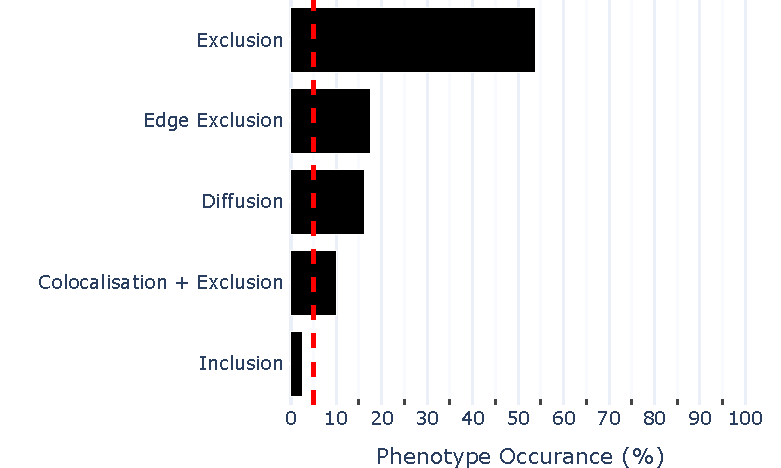
\includegraphics[width=1\linewidth]{08. Chapter 3/Figs/02. Infection/03. IFIT3/01. bar_i3_a549.pdf} 
    \end{subfigure}
    \begin{subfigure}{0.495\textwidth}
        \caption{}
        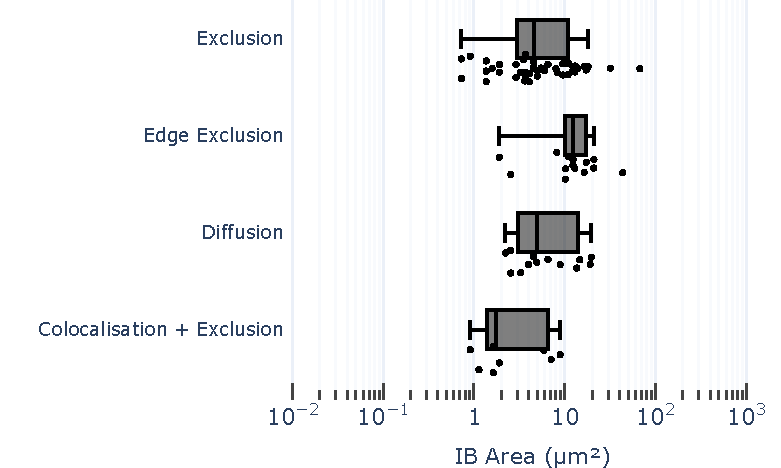
\includegraphics[width=1\linewidth]{08. Chapter 3/Figs/02. Infection/03. IFIT3/02. box_i3_a549.pdf}
    \end{subfigure}
    \caption[Phenotypic Diversity of hIFIT3 Interactions with hRSV Inclusion Bodies in A549 Cell Line.]{\textbf{Phenotypic Diversity of hIFIT3 Interactions with hRSV Inclusion Bodies in A549 Cell Line.} A549 cells were infected with human RSV at MOI 1 and fixed 24 HPI. Cells were double-labeled with with anti-RSV N and anti-IFIT3 antibodies and imaged on confocal microscope. Panel (a) shows percentual proportions of observed phenotypes between hRSV inclusion bodies and hIFIT3 (80 observations), with the red dotted line denoting the 5\% threshold, marking phenotypes considered relevant above this limit. Panel (b) shows the IB area in \(\mu \mbox{m}^2\) per observed relevant phenotype.}
    \label{fig:Phenotypic Diversity of hIFIT3 Interactions with hRSV Inclusion Bodies in A549 Cell Line}
\end{figure}

\begin{figure}
    \centering
    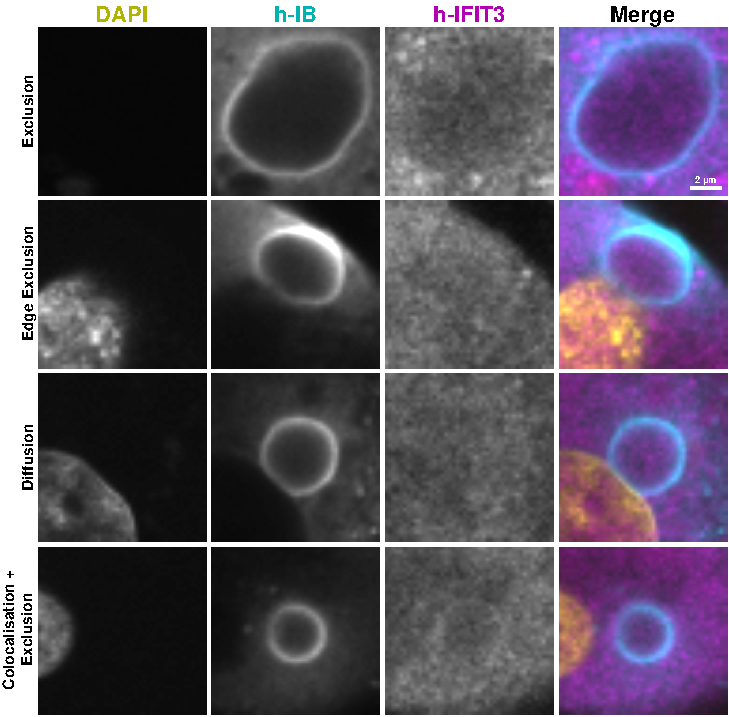
\includegraphics[width=1\linewidth]{08. Chapter 3/Figs/02. Infection/03. IFIT3/03. a549 i3.pdf}
    \caption[Representative Images of Phenotypic Diversity of hIFIT3 Interactions with hRSV Inclusion Bodies in A549 Cell Line.]{\textbf{Representative Images of Phenotypic Diversity of hIFIT3 Interactions with hRSV Inclusion Bodies in A549 Cell Line.} A549 cells were infected with hRSV at MOI 1 and fixed at 24 HPI. Cellular nuclei were stained with DAPI (yellow), and cells were double-labeled with anti-RSV N (cyan) and anti-IFIT3 (magenta) antibodies. This figure showcases representative examples of relevant phenotypes in the interaction between hIFIT3 and hRSV inclusion bodies. These phenotypes are presented in descending order based on their percentage proportions. The scale bar indicates 2 \(\mu \mbox{m}\).}
    \label{fig:Representative Images of Phenotypic Diversity of hIFIT3 Interactions with hRSV Inclusion Bodies in A549 Cell Line}
\end{figure}

DESCRIBE IFIT3 BEAS2B

62, 19, 12

5.5, 3, 10, 2.3

\begin{figure}
    \begin{subfigure}{0.495\textwidth}
        \caption{}
        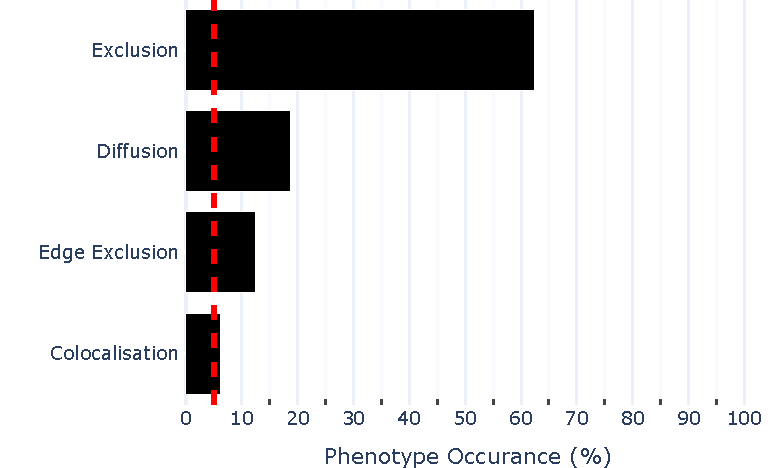
\includegraphics[width=1\linewidth]{08. Chapter 3/Figs/02. Infection/03. IFIT3/04. bar_i3_beas2b.pdf} 
    \end{subfigure}
    \begin{subfigure}{0.495\textwidth}
        \caption{}        
        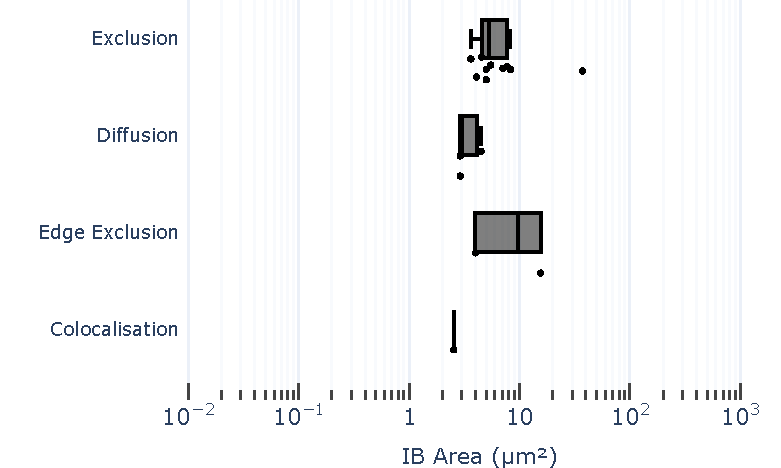
\includegraphics[width=1\linewidth]{08. Chapter 3/Figs/02. Infection/03. IFIT3/05. box_i3_beas2b.pdf}
    \end{subfigure}
    \caption[Phenotypic Diversity of hIFIT3 Interactions with hRSV Inclusion Bodies in BEAS2B Cell Line.]{\textbf{Phenotypic Diversity of hIFIT3 Interactions with hRSV Inclusion Bodies in BEAS2B Cell Line.} BEAS2B cells were infected with human RSV at MOI 1 and fixed 24 HPI. Cells were labeled with anti-RSV N and anti-IFIT3 antibodies and imaged on confocal microscope. Panel (a) shows percentual proportions of observed phenotypes between hRSV inclusion bodies and hIFIT3 (16 observations), with the red dotted line denoting the 5\% threshold, marking phenotypes considered relevant above this limit. Panel (b) shows the IB area in \(\mu \mbox{m}^2\) per observed relevant phenotype.}
    \label{fig:Phenotypic Diversity of hIFIT3 Interactions with hRSV Inclusion Bodies in BEAS2B Cell Line}
\end{figure}

\begin{figure}
    \centering
    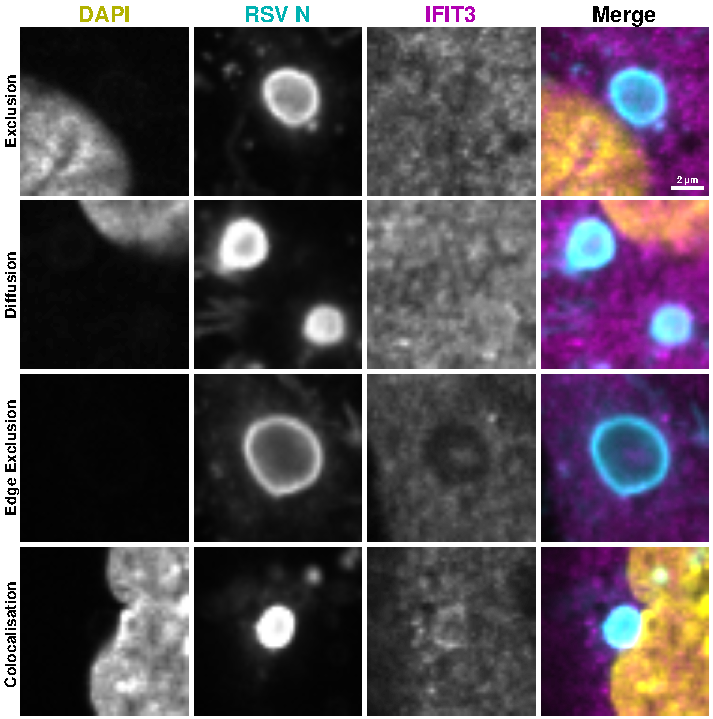
\includegraphics[width=1\linewidth]{08. Chapter 3/Figs/02. Infection/03. IFIT3/06. beas2b i3.pdf}
    \caption[Representative Images of Phenotypic Diversity of hIFIT3 Interactions with hRSV Inclusion Bodies in BEAS2B Cell Line]{\textbf{Representative Images of Phenotypic Diversity of hIFIT3 Interactions with hRSV Inclusion Bodies in BEAS2B Cell Line.} BEAS2B cells were infected with hRSV at MOI 1 and fixed at 24 HPI. Cellular nuclei were stained with DAPI (yellow), and cells were double-labeled with anti-RSV N (cyan) and anti-IFIT3 (magenta) antibodies. This figure showcases representative examples of relevant phenotypes in the interaction between hIFIT3 and hRSV inclusion bodies. These phenotypes are presented in descending order based on their percentage proportions. The scale bar indicates 2 \(\mu \mbox{m}\).}
    \label{fig:Representative Images of Phenotypic Diversity of hIFIT3 Interactions with hRSV Inclusion Bodies in BEAS2B Cell Line}
\end{figure}

DESCRIBE IFIT3 MDBK

43, 34, 11, 8

1.1, 3.3, 1, 11

PUT ALL 3 CELLINES IFIT3 TOGETHER

\begin{figure}
    \begin{subfigure}{0.495\textwidth}
        \caption{}
        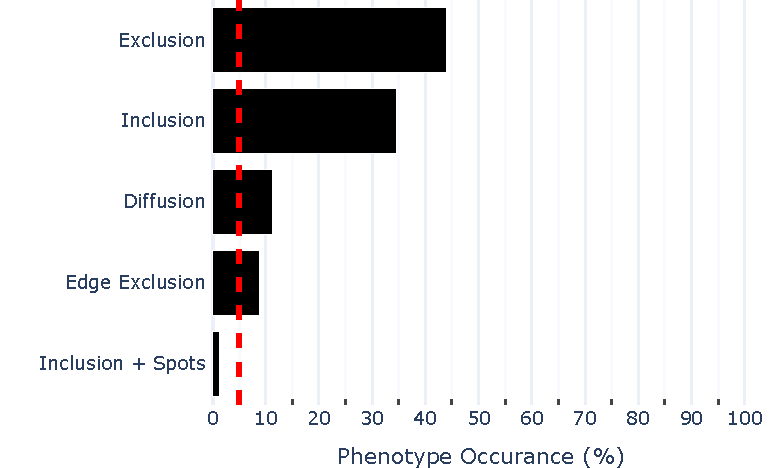
\includegraphics[width=1\linewidth]{08. Chapter 3/Figs/02. Infection/03. IFIT3/07. bar_i3_mdbk.pdf} 
    \end{subfigure}
    \begin{subfigure}{0.495\textwidth}
        \caption{}
        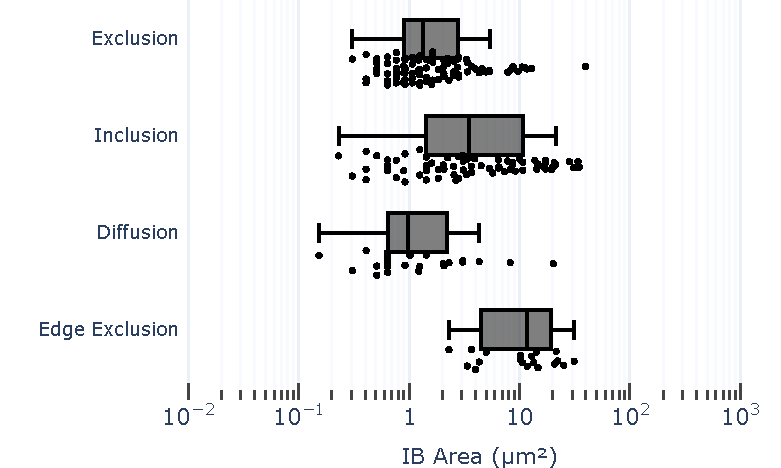
\includegraphics[width=1\linewidth]{08. Chapter 3/Figs/02. Infection/03. IFIT3/08. box_i3_mdbk.pdf}
    \end{subfigure}
    \caption[Phenotypic Diversity of bIFIT3 Interactions with bRSV Inclusion Bodies in MDBK Cell Line.]{\textbf{Phenotypic Diversity of bIFIT3 Interactions with bRSV Inclusion Bodies in MDBK Cell Line.} MDBK cells were infected with bovine RSV at MOI 1 and fixed 24 HPI. Cells were labeled with anti-RSV N and anti-IFIT3 antibodies and imaged on confocal microscope. Panel (a) shows percentual proportions of observed phenotypes between bRSV inclusion bodies and bIFIT3 (214 observations), with the red dotted line denoting the 5\% threshold, marking phenotypes considered relevant above this limit. Panel (b) shows the IB area in \(\mu \mbox{m}^2\) per observed relevant phenotype.}
    \label{fig:Phenotypic Diversity of bIFIT3 Interactions with bRSV Inclusion Bodies in MDBK Cell Line}
\end{figure}

\begin{figure}
    \centering
    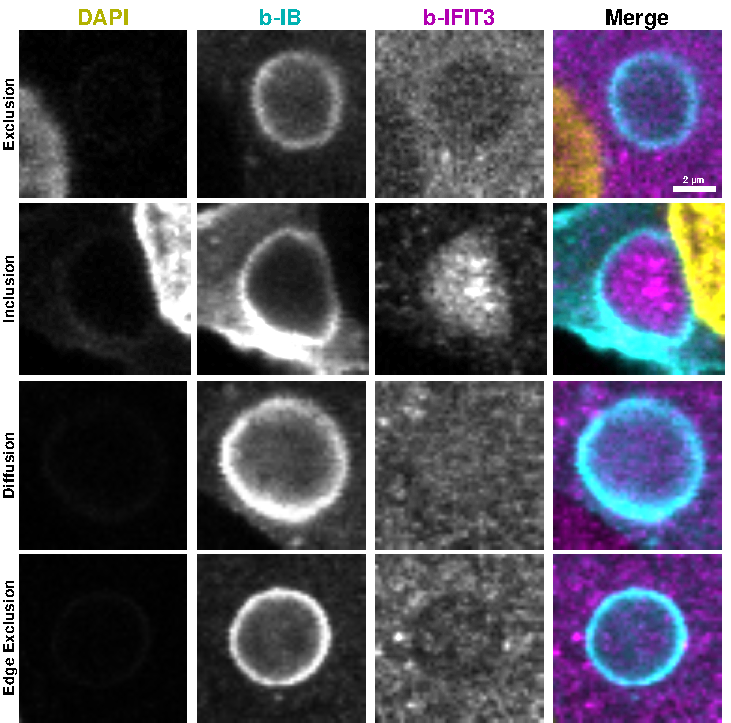
\includegraphics[width=1\linewidth]{08. Chapter 3/Figs/02. Infection/03. IFIT3/09. mdbk i3.pdf}
    \caption[Representative Images of Phenotypic Diversity of bIFIT3 Interactions with bRSV Inclusion Bodies in MDBK Cell Line.]{\textbf{Representative Images of Phenotypic Diversity of bIFIT3 Interactions with bRSV Inclusion Bodies in MDBK Cell Line.} MDBK cells were infected with bRSV at MOI 1 and fixed at 24 HPI. Cellular nuclei were stained with DAPI (yellow), and cells were double-labeled with anti-RSV N (cyan) and anti-IFIT3 (magenta) antibodies. This figure showcases representative examples of relevant phenotypes in the interaction between bIFIT3 and bRSV inclusion bodies. These phenotypes are presented in descending order based on their percentage proportions. The scale bar indicates 2 \(\mu \mbox{m}\).}
    \label{fig:Representative Images of Phenotypic Diversity of bIFIT3 Interactions with bRSV Inclusion Bodies in MDBK Cell Line}
\end{figure}

\subsubsection{Phenotypic Diversity of Nascent IFIT5 Interaction with RSV Inclusion Bodies}

DECRIBE IFIT5 A549

58, 17, 16, 5

6.3, 4, 8, 13

\begin{figure}
    \begin{subfigure}{0.495\textwidth}
        \caption{}
        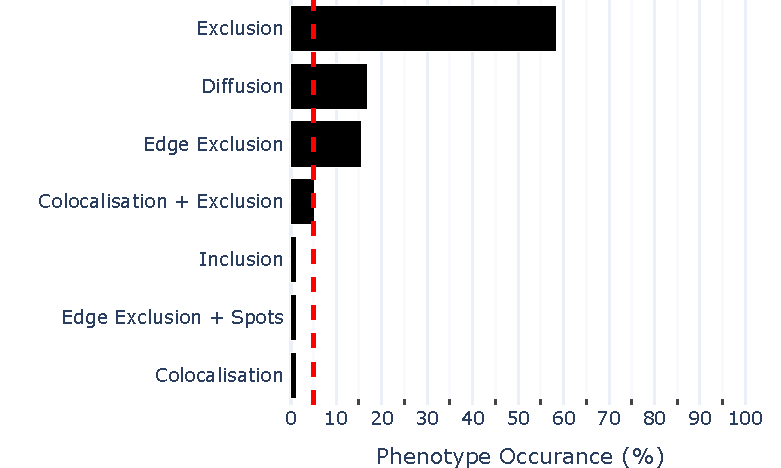
\includegraphics[width=1\linewidth]{08. Chapter 3/Figs/02. Infection/04. IFIT5/01. bar_i5_a549.pdf} 
    \end{subfigure}
    \begin{subfigure}{0.495\textwidth}
        \caption{}
        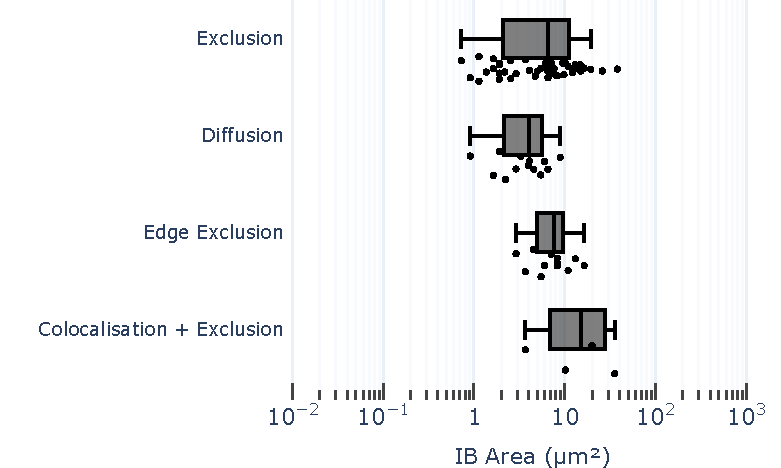
\includegraphics[width=1\linewidth]{08. Chapter 3/Figs/02. Infection/04. IFIT5/02. box_i5_a549.pdf}
    \end{subfigure}
    \caption[Phenotypic Diversity of hIFIT5 Interactions with hRSV Inclusion Bodies in A549 Cell Line.]{\textbf{Phenotypic Diversity of hIFIT5 Interactions with hRSV Inclusion Bodies in A549 Cell Line.} A549 cells were infected with human RSV at MOI 1 and fixed 24 HPI. Cells were labeled with anti-RSV N and anti-IFIT5 antibodies and imaged on confocal microscope. Panel (a) shows percentual proportions of observed phenotypes between hRSV inclusion bodies and hIFIT5 (77 observations), with the red dotted line denoting the 5\% threshold, marking phenotypes considered relevant above this limit. Panel (b) shows the IB area in \(\mu \mbox{m}^2\) per observed relevant phenotype.}
    \label{fig:Phenotypic Diversity of hIFIT5 Interactions with hRSV Inclusion Bodies in A549 Cell Line}
\end{figure}

\begin{figure}
    \centering
    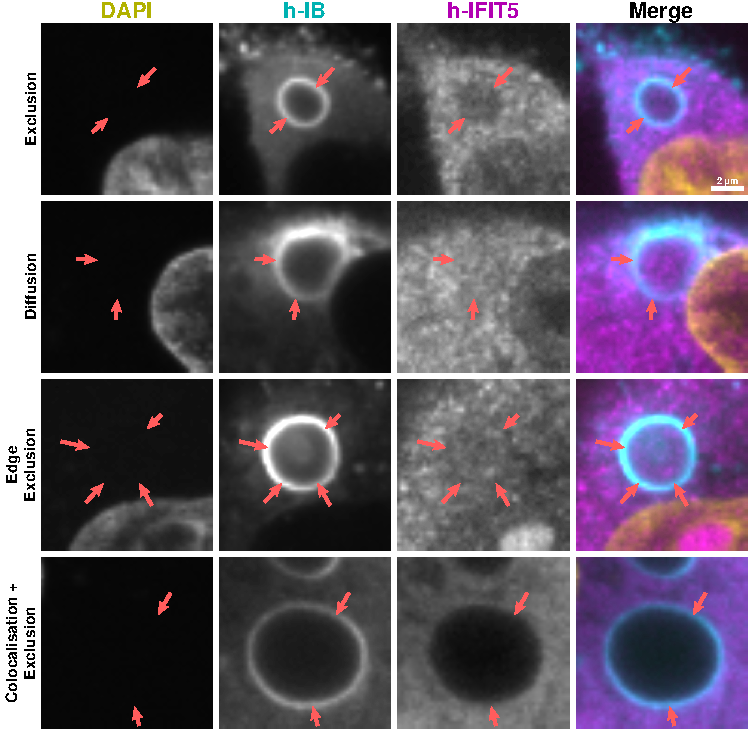
\includegraphics[width=1\linewidth]{08. Chapter 3/Figs/02. Infection/04. IFIT5/03. a549 i5.pdf}
    \caption[Representative Images of Phenotypic Diversity of hIFIT5 Interactions with hRSV Inclusion Bodies in A549 Cell Line.]{\textbf{Representative Images of Phenotypic Diversity of hIFIT5 Interactions with hRSV Inclusion Bodies in A549 Cell Line.} A549 cells were infected with hRSV at MOI 1 and fixed at 24 HPI. Cellular nuclei were stained with DAPI (yellow), and cells were double-labeled with anti-RSV N (cyan) and anti-IFIT5 (magenta) antibodies. This figure showcases representative examples of relevant phenotypes in the interaction between hIFIT5 and hRSV inclusion bodies. These phenotypes are presented in descending order based on their percentage proportions. The scale bar indicates 2 \(\mu \mbox{m}\).}
    \label{fig:Representative Images of Phenotypic Diversity of hIFIT5 Interactions with hRSV Inclusion Bodies in A549 Cell Line}
\end{figure}

DESCRIBE IFIT5 BEAS2B

62, 18, 18

2, 2.3, 3

\begin{figure}
    \begin{subfigure}{0.495\textwidth}
        \caption{}
        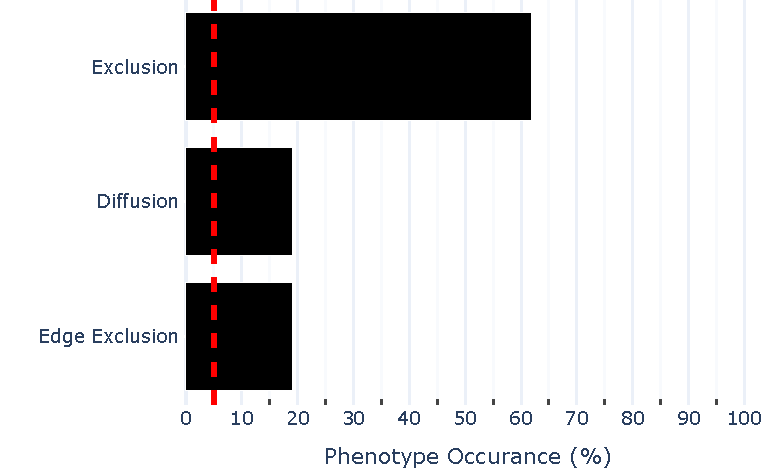
\includegraphics[width=1\linewidth]{08. Chapter 3/Figs/02. Infection/04. IFIT5/04. bar_i5_beas2b.pdf}
    \end{subfigure}
    \begin{subfigure}{0.495\textwidth}
        \caption{}
        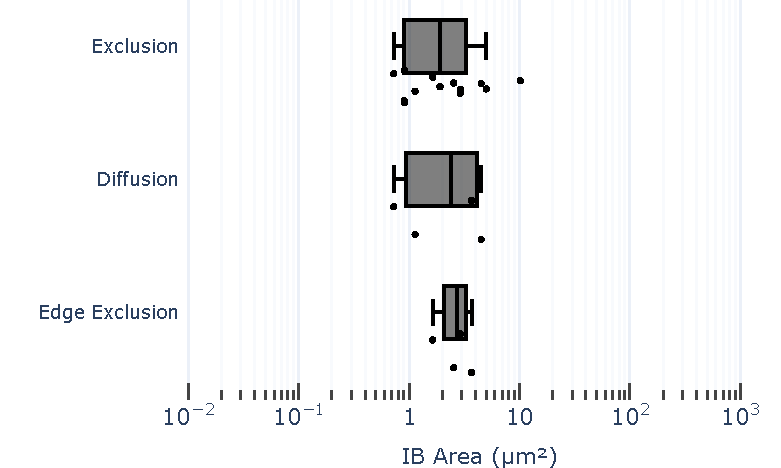
\includegraphics[width=1\linewidth]{08. Chapter 3/Figs/02. Infection/04. IFIT5/05. box_i5_beas2b.pdf}
    \end{subfigure}
    \caption[Phenotypic Diversity of hIFIT5 Interactions with hRSV Inclusion Bodies in BEAS2B Cell Line.]{\textbf{Phenotypic Diversity of hIFIT5 Interactions with hRSV Inclusion Bodies in BEAS2B Cell Line.} BEAS2B cells were infected with human RSV at MOI 1 and fixed 24 HPI. Cells were labeled with anti-RSV N and anti-IFIT5 antibodies and imaged on confocal microscope. Panel (a) shows percentual proportions of observed phenotypes between hRSV inclusion bodies and hIFIT5 (21 observations), with the red dotted line denoting the 5\% threshold, marking phenotypes considered relevant above this limit. Panel (b) shows the IB area in \(\mu \mbox{m}^2\) per observed relevant phenotype.}
    \label{fig:Phenotypic Diversity of hIFIT5 Interactions with hRSV Inclusion Bodies in BEAS2B Cell Line}
\end{figure}

\begin{figure}
    \centering
    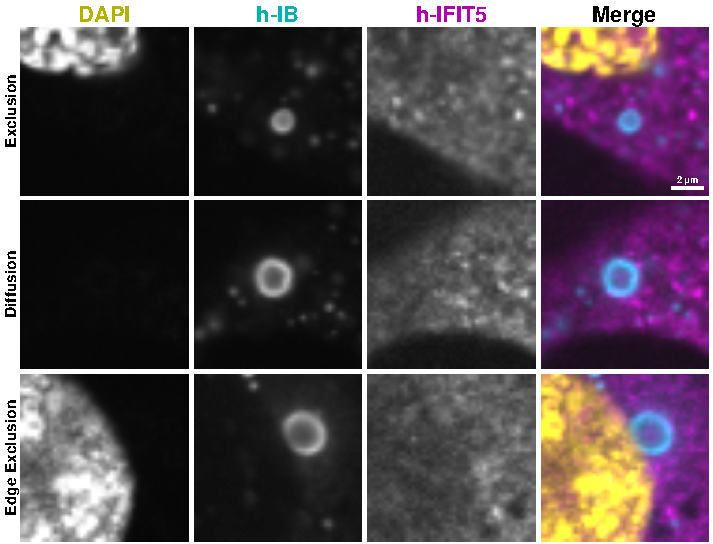
\includegraphics[width=1\linewidth]{08. Chapter 3/Figs/02. Infection/04. IFIT5/06. beas2b i5.pdf}
    \caption[Representative Images of Phenotypic Diversity of hIFIT5 Interactions with hRSV Inclusion Bodies in BEAS2B Cell Line.]{\textbf{Representative Images of Phenotypic Diversity of hIFIT5 Interactions with hRSV Inclusion Bodies in BEAS2B Cell Line.} BEAS2B cells were infected with hRSV at MOI 1 and fixed at 24 HPI. Cellular nuclei were stained with DAPI (yellow), and cells were double-labeled with anti-RSV N (cyan) and anti-IFIT5 (magenta) antibodies. This figure showcases representative examples of relevant phenotypes in the interaction between hIFIT5 and hRSV inclusion bodies. These phenotypes are presented in descending order based on their percentage proportions. The scale bar indicates 2 \(\mu \mbox{m}\).}
    \label{fig:Representative Images of Phenotypic Diversity of hIFIT5 Interactions with hRSV Inclusion Bodies in BEAS2B Cell Line}
\end{figure}

DESCRIBE IFIT5 MDBK

51, 29, 10, 7

1, 10, 3, 0.9

PUT ALL CELLINES TOGETHER IFIT5

\begin{figure}
    \begin{subfigure}{0.495\textwidth}
        \caption{}
        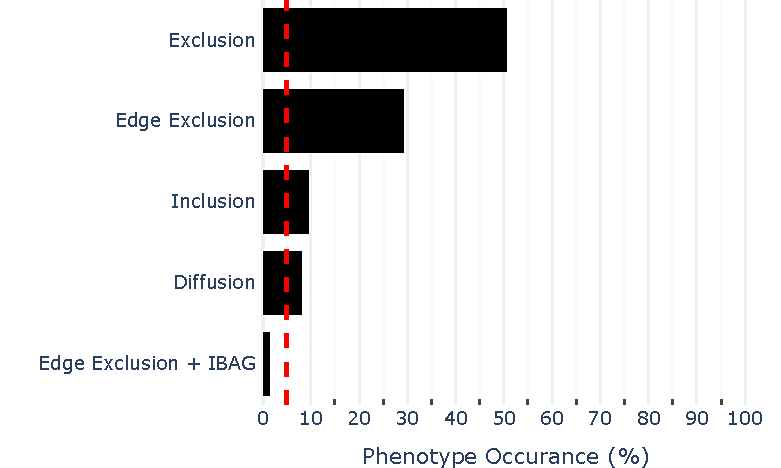
\includegraphics[width=1\linewidth]{08. Chapter 3/Figs/02. Infection/04. IFIT5/07. bar_i5_mdbk.pdf} 
    \end{subfigure}
    \begin{subfigure}{0.495\textwidth}
        \caption{}
        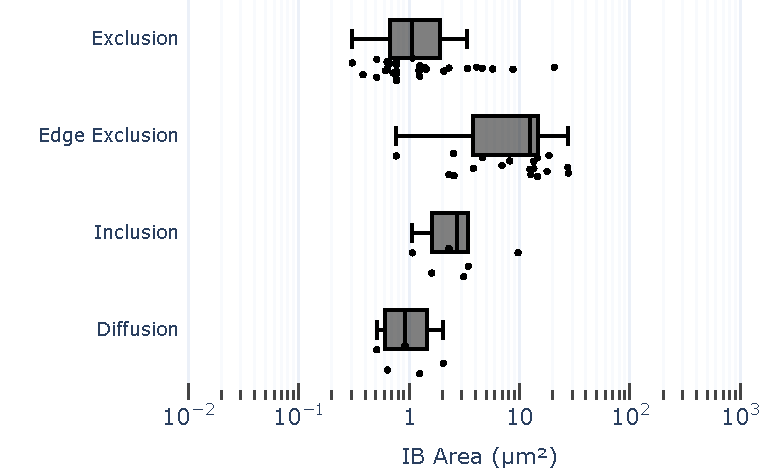
\includegraphics[width=1\linewidth]{08. Chapter 3/Figs/02. Infection/04. IFIT5/08. box_i5_mdbk.pdf}
    \end{subfigure}
    \caption[Phenotypic Diversity of bIFIT5 Interactions with bRSV Inclusion Bodies in MDBK Cell Line.]{\textbf{Phenotypic Diversity of bIFIT5 Interactions with bRSV Inclusion Bodies in MDBK Cell Line.} MDBK cells were infected with bovine RSV at MOI 1 and fixed 24 HPI. Cells were labeled with anti-RSV N and anti-IFIT5 antibodies and imaged on confocal microscope. Panel (a) shows percentual proportions of observed phenotypes between bRSV inclusion bodies and bIFIT5 (61 observations), with the red dotted line denoting the 5\% threshold, marking phenotypes considered relevant above this limit. Panel (b) shows the IB area in \(\mu \mbox{m}^2\) per observed relevant phenotype.}
    \label{fig:Phenotypic Diversity of bIFIT5 Interactions with bRSV Inclusion Bodies in MDBK Cell Line}
\end{figure}

\begin{figure}
    \centering
    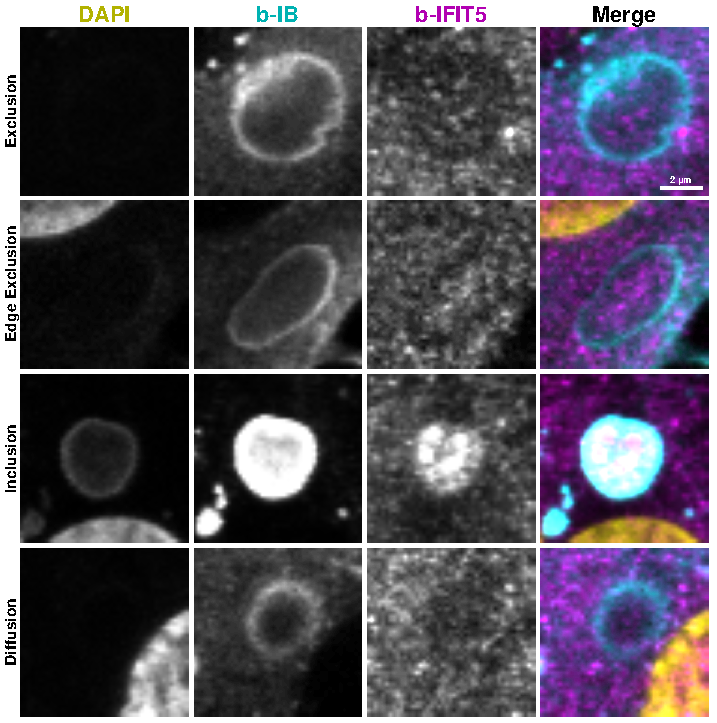
\includegraphics[width=1\linewidth]{08. Chapter 3/Figs/02. Infection/04. IFIT5/09. mdbk i5.pdf}
    \caption[Representative Images of Phenotypic Diversity of bIFIT5 Interactions with bRSV Inclusion Bodies in MDBK Cell Line.]{\textbf{Representative Images of Phenotypic Diversity of bIFIT5 Interactions with bRSV Inclusion Bodies in MDBK Cell Line.} MDBK cells were infected with bRSV at MOI 1 and fixed at 24 HPI. Cellular nuclei were stained with DAPI (yellow), and cells were double-labeled with anti-RSV N (cyan) and anti-IFIT5 (magenta) antibodies. This figure showcases representative examples of relevant phenotypes in the interaction between bIFIT5 and bRSV inclusion bodies. These phenotypes are presented in descending order based on their percentage proportions. The scale bar indicates 2 \(\mu \mbox{m}\).}
    \label{fig:Representative Images of Phenotypic Diversity of bIFIT5 Interactions with bRSV Inclusion Bodies in MDBK Cell Line}
\end{figure}

PUT ALL IFITS TOGETHER

HYPOTHETISE ABOUT INTERACTION BETWEEN IFITS AND IB maturity

SAY ABOUT THE NEXT STEPS WITH pIB AS A SIMPLIFIED SYSTEM THAT COULD ANDWER THE DIVERSITY QUESTION

